\chapter{对流传热理论分析与实验研究基础}
\thispagestyle{empty}
\section{对流传热概述}

\subsection{对流传热的影响因素}
\noindent 影响对流传热的因素就是影响流动的因素及影响流体中热量传递的因素,可以归结为五个方面
\begin{itemize}
	\item 流体流动的起因
\vspace*{-0.5em}
	\item 流体有无相变
\vspace*{-0.5em}
	\item 流体的流动状态
\vspace*{-0.5em}
	\item 传热表面的几何因素
\vspace*{-0.5em}
	\item 流体的物理性质
\end{itemize}
\vspace*{0.5em}

\subsection{对流传热现象 分类}
\begin{equation*}
	\begin{cases}
		\, \mbox{\dy[无相变对流传热]{WXBDLCR}}\,
		\begin{cases}
			\, \mbox{\dy[自然对流传热]{ZRDLCR}}
			\begin{cases}
				\, \mbox{大空间自然对流传热}\\
				\, \mbox{有限空间自然对流传热}
			\end{cases}\\[2em]
			\, \mbox{\dy[强制对流传热]{QZDLCR}}
			\begin{cases}
				\, \mbox{内部流动强制对流传热}\\
				\, \mbox{外部流动强制对流传热}
			\end{cases}\\
			\, \mbox{\dy[混合对流传热]{HHDLCR}}
		\end{cases}
		\\[6em]
		\, \mbox{\dy[有相变对流传热]{YXBDLCR}}
		\begin{cases}
			\, \mbox{\dy[沸腾传热]{FTCR}}
			\begin{cases}
				\, \mbox{大容器沸腾传热}\\
				\, \mbox{管内沸腾传热}
			\end{cases}\\[2em]
			\, \mbox{\dy[凝结传热]{NJCR}}
			\begin{cases}
				\, \mbox{管外凝结传热}\\
				\, \mbox{管内凝结传热}
			\end{cases}
		\end{cases}
	\end{cases}
\end{equation*}

\subsection{对流传热的研究方法}
对流传热的研究方法主要有四种:分析法、实验法、比拟法、数值法。

\noindent \textbf{1. 分析法}

分析法是指对描述某一类对流传热问题的偏微分方程及相应的定解条件进行数学求解,从而获得速度场和温度场的分析解的方法。\index{FXF@分析法}

\noindent \textbf{2. 实验法}

实验法是指在相似原理指导下通过实验获得表面传热系数的计算式的方法。\index{SYF@实验法}

\noindent \textbf{3. 比拟法}

比拟法是指通过研究动量传递及热量传递的共性或类似特性,以建立起表面传热系数与阻力系数间的相互关系的方法。\index{BNF@比拟法}

\noindent \textbf{4. 数值法}

数值法是指通过计算机获得某个计算条件下物体中代表性空间点上的速度值和温度值的方法。\index{SZF@数值法}
\vspace*{1em}

\subsection{通过流体温度场计算表面传热系数}
当黏性流体在壁面上流动时,由于黏性的作用,在靠近壁面的地方流速逐渐减小,而在贴壁处流体将被滞止而处于无滑移状态。也就是说,贴壁处这一极薄的流体层相对于壁面是不流动的
,这个条件称为\dy[无滑移边界条件]{WHYBJTJ}。穿过不流动的流体层的热量传递方式只能是导热。

壁面的总换热量等于对流及辐射热量之和。不考虑辐射传热,对流传热就等于贴壁流体层的导热量,即
\begin{equation}
	q = - \lambda \dfrac{\partial t}{\partial y} \Bigg|_{y=0}
\end{equation}
由牛顿冷却定律
\begin{equation}
	q = h \Delta t
\end{equation}
联立得到
\begin{equation}
	h = - \dfrac{\lambda}{\Delta t} \dfrac{\partial t}{\partial y}\Bigg|_{y = 0}
\end{equation}
其中,$h$为表面传热系数,$\lambda$为\dy[流体导热系数]{LTDRXS},$t$为流体温度。


\section{对流传热问题的数学描述}
\subsection{运动流体能量方程}
\noindent \textbf{1. 简化假设}
\begin{enumerate}[\hspace*{2em} (1) ]
	\item 流体为牛顿型流体
\vspace*{-0.5em}
	\item 流动是二维的
\vspace*{-0.5em}
	\item 流动是不可压缩的
\vspace*{-0.5em}
	\item 常热物性
\vspace*{-0.5em}
	\item 无内热源
\vspace*{-0.5em}
	\item 粘性耗散产生的耗散热可以忽略不计
\end{enumerate}

\noindent \textbf{2. 微元体能量平衡分析}

由热力学第一定律,得
\begin{equation}
	\varPhi = \dfrac{\d E_{\text{C.V}}}{\d \tau} + \big(q_m\big)_{\text{out}} \left(h + \dfrac{1}{2}v^2 + gz\right)_{\text{out}} - \big(q_m\big)_{\text{in}} \left(h + \dfrac{1}{2} v^2 + gz\right)_{\text{in}} + W_{\text{net}}
\end{equation}
其中,$q_m$为质量流量;$h$为流体的比焓;下标in和out分别对应流入系统的流体和流出系统的流体;$\d E_{\text{C.V}}$为微元控制体增加的能量;$\varPhi$为通过界面由外界导入微元体的热流量;$W_{\text{net}}$为流体所作的净功。

由于流体位能及动能变化小,也不考虑作功,得
\begin{equation}
	\varPhi = \dfrac{\d U}{\d \tau} + \big(q_m\big)_{\text{out}}h_{\text{out}}-\big(q_m\big)_{\text{in}}h_{\text{in}}
\end{equation}
\begin{figure}[!htb]
	\centering
	\vspace*{-2em}
	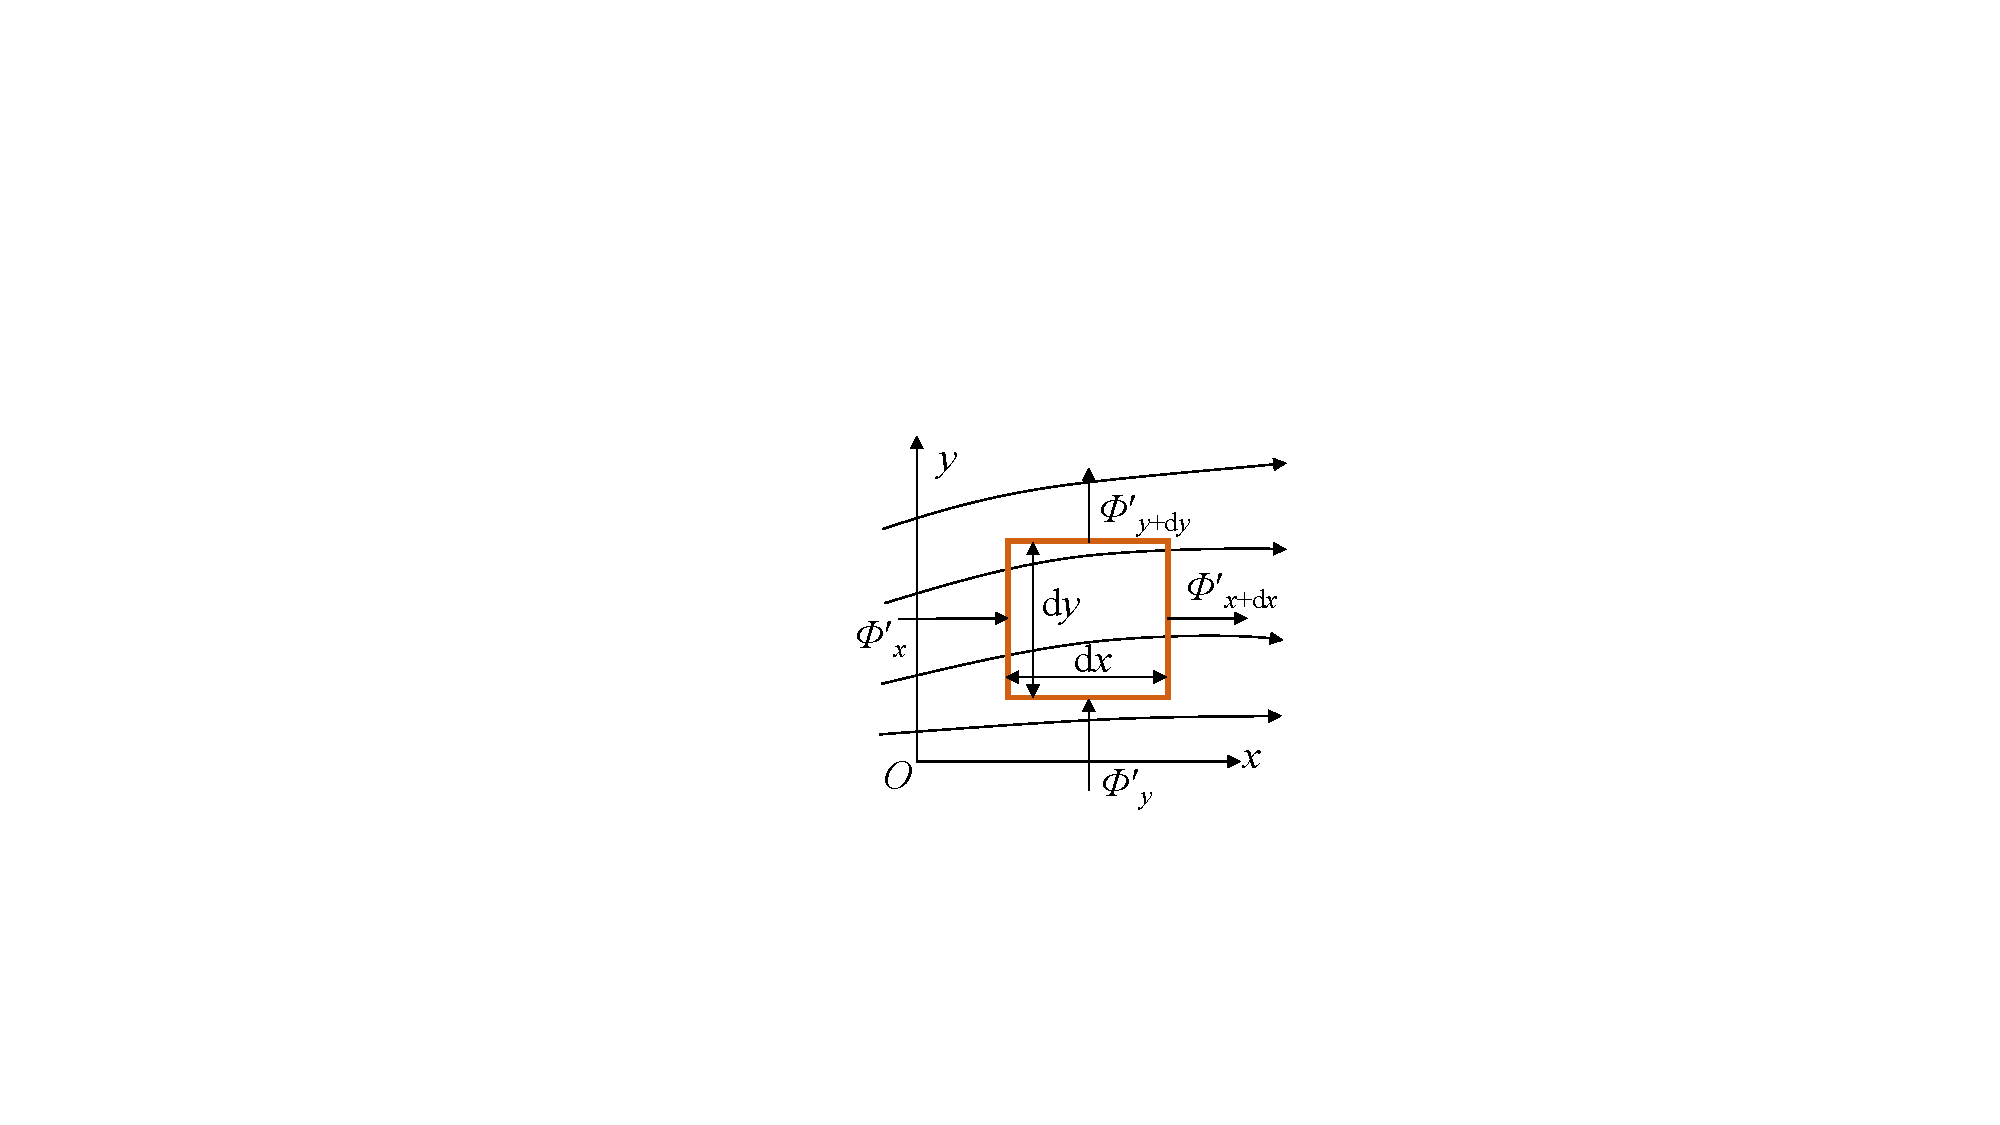
\includegraphics[width=0.25\linewidth]{pic/微元体能量平衡.pdf}
	\vspace*{-1em}
	\caption{微元体能量平衡示意图}
	\label{微元体能量平衡}
\end{figure}

所以$\d \tau$时间内导热进入微元体的热量为
\begin{equation}
	\varPhi \, \d \tau = \lambda \left(\dfrac{\partial^2 t}{\partial x^2} + \dfrac{\partial^2 t}{\partial y^2}\right) \, \d x \d y \d \tau
\end{equation}

微元体热力学能的增量为
\begin{equation}
	\d U = \rho \, \d x \d y c \dfrac{\partial t}{\partial \tau}\, \d \tau
	\label{能量守恒分析}
\end{equation}
$x$截面流入微元体的焓为
\begin{equation}
	\bigg[\big(q_m\big)_{\text{in}}h_{\text{in}}\bigg]_x \, \d \tau = H_x = mct = \rho S c t = \rho u \, \d y \, ct \, \d \tau
\end{equation}
$x + \d x$截面流入微元体的焓为
\begin{equation}
	\bigg[\big( q_m \big)_{\text{out}} h_{\text{out}}\bigg]_{x+\d x} \, \d \tau = H_{x +\d x} = \rho \left(u+\dfrac{\partial u}{\partial x}\, \d x\right) \, \d y \, c \left(t + \dfrac{\partial t}{\partial x}\, \d x\right) \d \tau
\end{equation}

$x$方向流体净带出微元体的焓为
\begin{equation}
	\bigg[\big( q_m \big)_{\text{out}} h_{\text{out}} -\big(q_m \big)_{\text{in}} h_{\text{in}} \bigg]_{x} \, \d \tau = H_{x + \d x} - H_x = \rho c \left(u \dfrac{\partial t}{\partial x} + t \dfrac{\partial u}{\partial x}\right)\, \d x \d y \d \tau
\end{equation}

同理可得$y$方向流体净带出微元体的焓为
\begin{equation}
	\bigg[\big( q_m \big)_{\text{out}} h_{\text{out}} -\big(q_m\_{\text{in}} \big) h_{\text{in}} \bigg]_{y} \, \d \tau = H_{y + \d y} - H_y = \rho c \left(v \dfrac{\partial t}{\partial y} + t \dfrac{\partial u}{\partial y}\right)\, \d x \d y \d \tau
\end{equation}

由不可压缩流体质量守恒方程
\begin{equation}
	\dfrac{\partial u}{\partial x} + \dfrac{\partial v}{\partial y} = 0
\end{equation}
可得
\begin{equation}
		\bigg[\big( q_m \big)_{\text{out}} h_{\text{out}} -\big(q_m\_{\text{in}} \big) h_{\text{in}} \bigg]_{y} \, \d \tau = \rho c \left(u \dfrac{\partial t}{\partial x} + v \dfrac{\partial t}{\partial y}\right)\, \d x \d y \d \tau
\end{equation}

所有项代入\eqref{能量守恒分析},可得\dy[运动流体能量方程]{YDLTNLFC}
\begin{equation}
	\dfrac{\partial t}{\partial \tau} + u \dfrac{\partial t}{\partial x} + v \dfrac{\partial t}{\partial y} = \dfrac{\lambda}{\rho c}\left(\dfrac{\partial^2 t}{\partial x^2} + \dfrac{\partial^2 t}{\partial y^2}\right)
	\label{运动流体}
\end{equation}
其中,$t(x,y,\tau)$是温度函数,$\tau$是时间,$u$是流体在$x$方向上的速度,$v$是流体在$y$方向上的速度,$\rho$是二维微元体的面密度,$c$是比定压热容,$\lambda $是导热系数。
\clearpage

\noindent \textbf{3. 运动流体能量方程的讨论}
\begin{enumerate}[\hspace*{2em}(1) ]
	\item 各项的物理意义
	\begin{itemize}
		\item $\dfrac{\partial t}{\partial \tau}$\quad 流体温度随时间的变化,称为非稳态项
		\vspace*{0.5em}
		\item $u\dfrac{\partial t}{\partial x}+v\dfrac{\partial t}{\partial y}$\quad 流体流出与流入控制容积净带走的热量,称为对流项
		\vspace*{0.5em}
		\item $\dfrac{\partial^2 t}{\partial x^2} + \dfrac{\partial^2 t}{\partial y^2}$\quad 流体热传导而净导入该控制容积的热量,称为扩散项
	\end{itemize}
	\item 这个方程表明:在流体运动过程中,热量的传递除了依靠流动(对流项所代表)以外,还有导热引起的扩散作用(扩散项所代表),即:运动着的流体除了依靠流体的宏观位移传递热量外,还依靠导热传递热量。
	
	\item 当流体静止时,方程\eqref{运动流体}退化为常热物性、无内热源的导热微分方程:
	\begin{equation}
		\dfrac{\partial t}{\partial \tau} = \dfrac{\lambda}{\rho c}\left(\dfrac{\partial^2 t}{\partial x^2} + \dfrac{\partial^2 t}{\partial y^2}\right)
	\end{equation}
	
	\item 稳态对流传热时,方程\eqref{运动流体}可写为
	\begin{equation}
		u \dfrac{\partial t}{\partial x} + v \dfrac{\partial t}{\partial y} = \dfrac{\lambda}{\rho c}\left(\dfrac{\partial^2 t}{\partial x^2} + \dfrac{\partial^2 t}{\partial y^2}\right)
	\end{equation}
	
	\item 如果流体中有内热源,其强度为$\dot{\varPhi}(x,y)$,则只要在上式右端加上$\dfrac{\dot{\varPhi}}{\rho c_\text{p}}$就得出有内热源的能量微分方程。\\
	
	特别的,对于二维常热物性流体,其粘性耗散所产生的内热源强度为
	\begin{equation}
		\varPhi(x,y) = \mu \Bigg\lbrace 2 \left[\left(\dfrac{\partial u}{\partial x}\right)^2 + \left(\dfrac{\partial v}{\partial y}\right)^2\right] + \left(\dfrac{\partial u}{\partial x} + \dfrac{\partial v}{\partial y}\right)^2 \Bigg\rbrace
	\end{equation}
	
\end{enumerate}

\subsection{对流传热问题的完整数学描述}
\noindent \textbf{1. 控制方程}
\begin{itemize}
	\item 质量守恒方程
	\begin{equation}
		\dfrac{\partial u}{\partial x} + \dfrac{\partial v}{\partial y}=0
	\end{equation}
	\item 动量守恒方程
	\begin{align}
		\rho \Bigg(\dfrac{\partial u}{\partial \tau} + u\dfrac{\partial u}{\partial x} + v\dfrac{\partial u}{\partial y}\Bigg) = F_x - \dfrac{\partial p}{\partial x} + \mu \Bigg(\dfrac{\partial^2 u }{\partial x^2} + \dfrac{\partial^2 u}{\partial y^2}\Bigg)\\[0.5em]
		\rho \Bigg(\dfrac{\partial u}{\partial \tau} + u\dfrac{\partial u}{\partial x} + v\dfrac{\partial u}{\partial y}\Bigg) = F_y - \dfrac{\partial p}{\partial y} + \mu \Bigg(\dfrac{\partial^2 u }{\partial x^2} + \dfrac{\partial^2 u}{\partial y^2}\Bigg)
	\end{align}
	\item 能量守恒方程
	\begin{equation}
		\dfrac{\partial t}{\partial \tau} + u \dfrac{\partial t}{\partial x} + v \dfrac{\partial t}{\partial y} = \dfrac{\lambda}{\rho c} \Bigg(\dfrac{\partial^2 t}{\partial x^2} + \dfrac{\partial^2 t}{\partial y^2}\Bigg)
	\end{equation}
\end{itemize}

\noindent \textbf{2. 定解条件}
\begin{itemize}
	\item 初始条件 \quad 初始时刻的速度、压力及温度
	\item 边界条件 \quad 边界上的速度、压力及温度
	\item 由于获得表面传热系数是求解对流传热问题的最终目的,一般地说求解对流传热问题时没有第三类边界条件。
\end{itemize}


\section{边界层型对流传热问题的数学描述}
\subsection{流动边界层及流动边界层动量方程}
\noindent \textbf{1. 普朗特的突破性见解}
\begin{itemize}
	\item 粘性起作用的区域仅仅局限在靠近壁面的薄层内
	\item 在此薄层以外的流动可作为理想流体的无旋流动
	\item 在这个粘性力不能忽略的薄层之内,运用数量级分析的方法可以对Navier-Stokes方程作实质性的简化,从而可以获得不少粘性流动问题的分析解
	\item 这种在固体表面附近流体速度发生剧烈变化的薄层称为\dy[流动边界层]{LDBJC},又称\dy[速度边界层]{SDBJC}
	
\end{itemize}

\noindent \textbf{2. 流动边界层}
\begin{figure}[!htb]
	\centering
	\vspace*{-1em}
	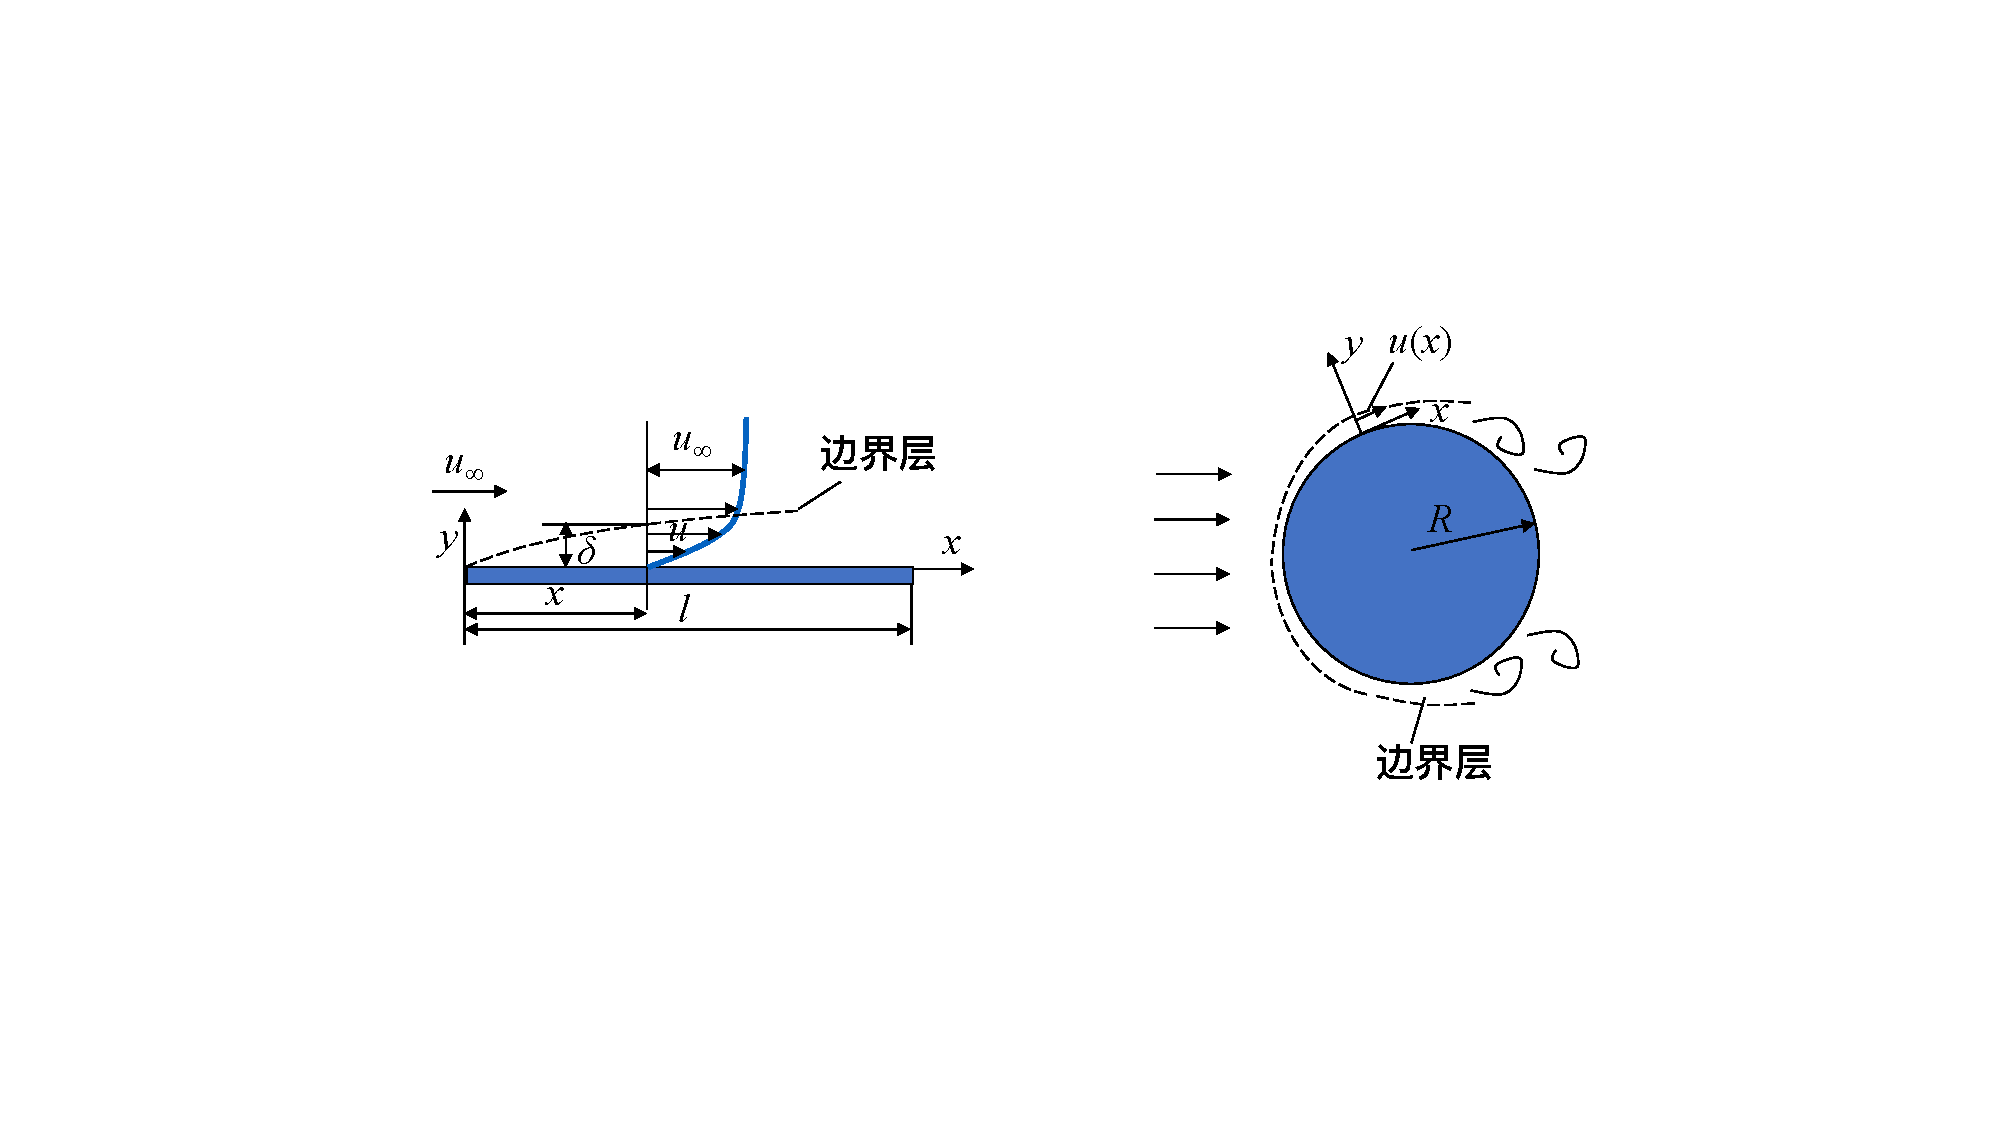
\includegraphics[width=0.65\linewidth]{pic/边界层.pdf}
	\vspace*{-1em}
	\caption{边界层}
	\label{边界层}
\end{figure}
\begin{enumerate}[\hspace*{2em} (1)]
	\item 流动边界层的定义\\
	从$y=0$处$u=0$开始,流体的速度随着离开壁面距离$y$的增加而急剧增大,经过一个薄层后$u$增长到接近主流速度,这个薄层即为\dy[流动边界层]{LDBJC}
。一般规定达到主流速度99\%处的距离$y$为流动边界层的厚度,记为$\delta$.
	
	\item 流动边界层的流态\\
	流动边界层内的流态包括层流和湍流两种。
	\begin{itemize}
		\item \dy[层流边界层]{CLBJC}\quad 流体有秩序的分层流动,各层互不干扰,边界层内的速度分布为抛物线形状
		\item \dy[湍流边界层]{TLBJC}\quad 湍流边界层是指流体质点沿$x$方向流动的同时,又作着紊乱的不规则脉动
		
		\begin{figure}[!htb]
			\centering
			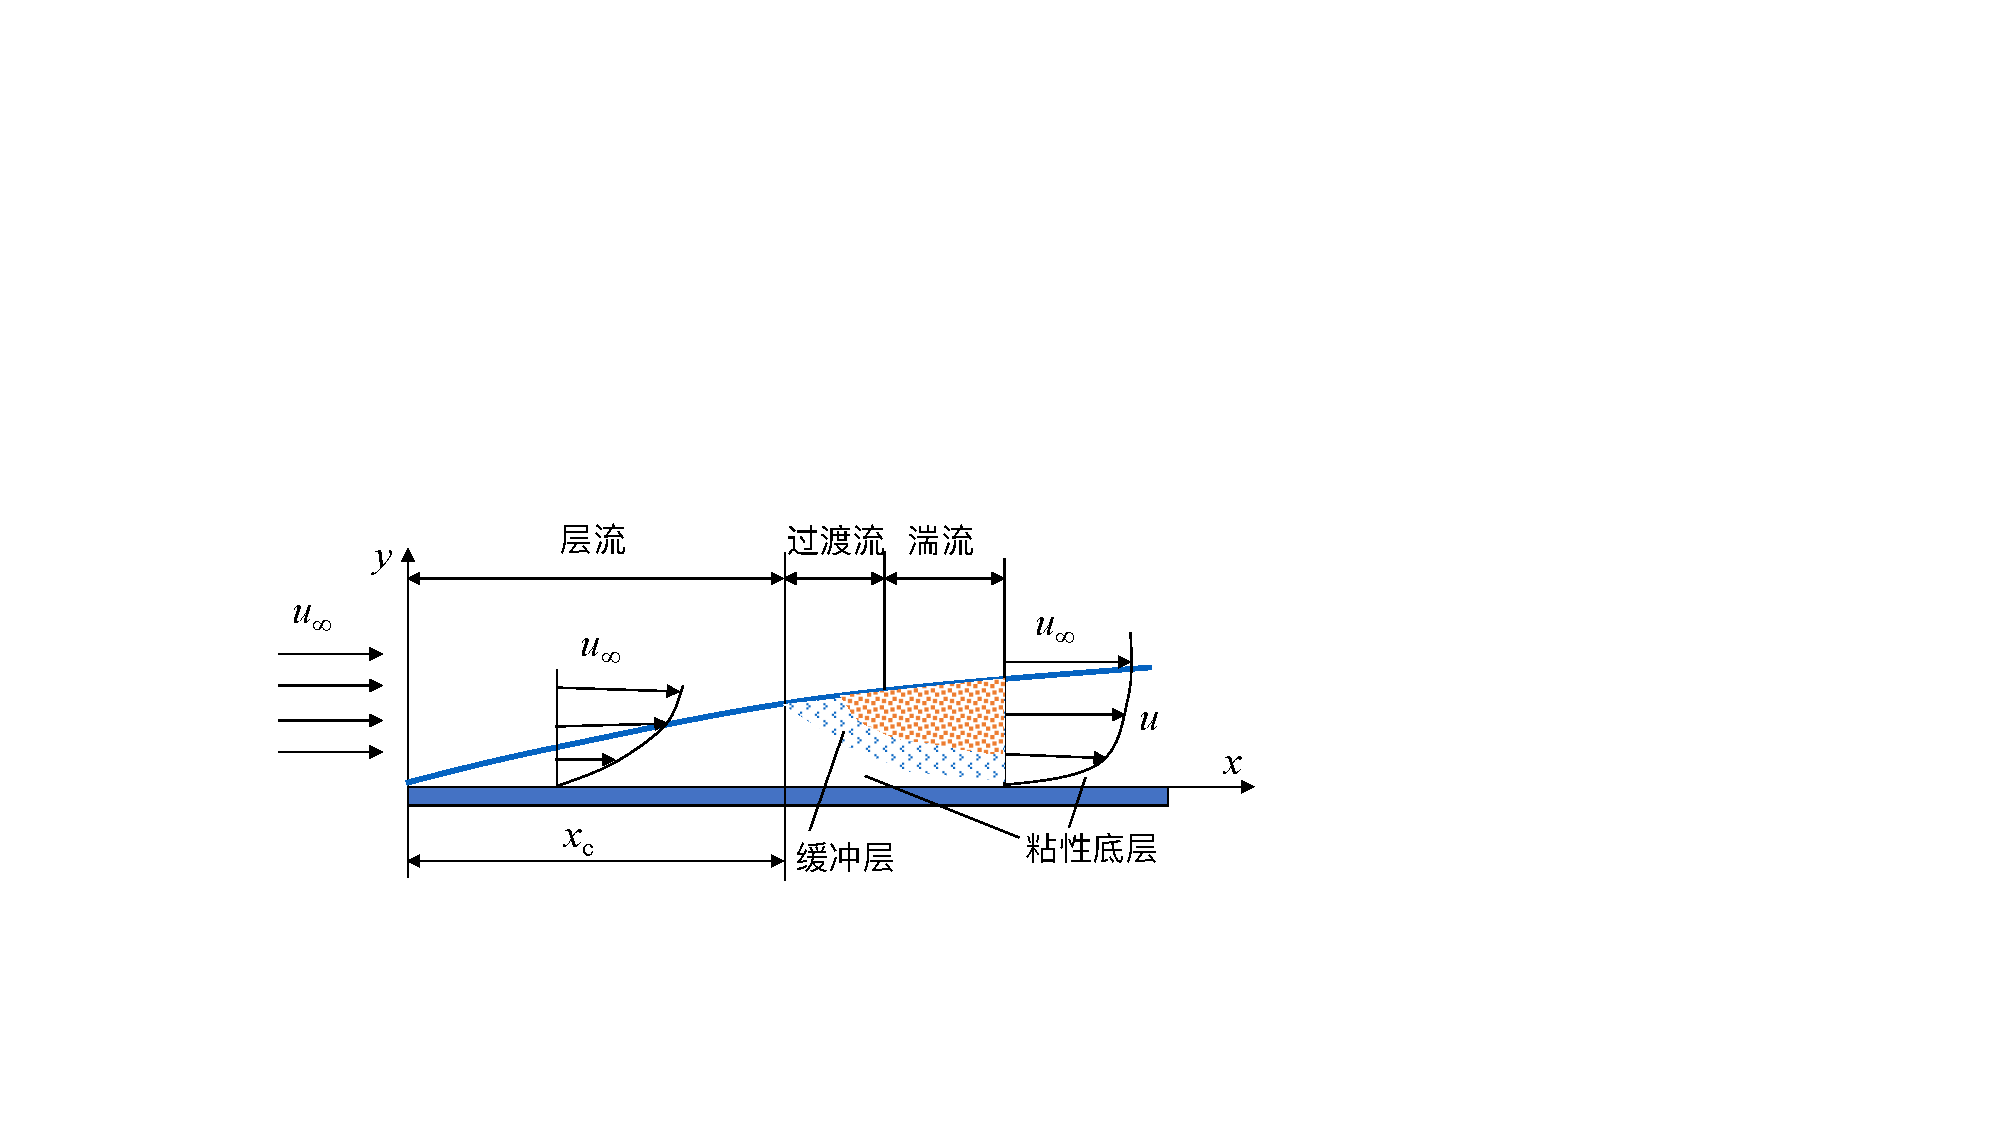
\includegraphics[width=0.6\linewidth]{pic/边界层的形成.pdf}
			\caption{掠过平板时边界层的形成和发展}
			\label{边界层的形成}
		\end{figure}
	
	\end{itemize}
		边界层由层流开始向湍流转变的距离由\dy[临界雷诺数]{LJRNS}确定:
		\begin{equation}
			Re_{\text{c}} = \dfrac{u_\infty x_\text{c}}{\nu} \approx 5 \times 10^5
		\end{equation}
	\hspace*{2em}湍流边界层的主体核心虽处于湍流状态,但紧靠壁面处粘性应力仍占主导地位,致使贴附于壁面的一极薄层内仍保持层流的主要性质,这个极薄层称为湍流边界层的\dy[黏性底层]{NXDC}。黏性底层的速度梯度较大,近于直线。在湍流核心,质点的脉动强化了动量传递,速度变化较为平缓。
\end{enumerate}

\noindent \textbf{3. 流动边界层内的动量方程}

层流边界层内的二维稳态不可压缩黏性流体动量方程为
\begin{align}
	u\dfrac{\partial u}{\partial x} + v \dfrac{\partial v}{\partial y} = - \dfrac{1}{\rho} \dfrac{\partial p}{\partial x} + \nu \left(\dfrac{\partial^2 u}{\partial x^2} + \dfrac{\partial^2 u}{\partial y^2}\right)
\end{align}
\begin{enumerate}[\hspace*{2em} (1)]
	\item 数量级分析的基本思想\\
	\dy[数量级分析]{SLJFX}指的是通过比较方程式中各项数量级的相对大小,把数量级较大的项保留下来,而舍去较小的项,实现方程式的合理简化。
	\item 实施方法\\
	对于流动边界层内的动量方程,采用各量在作用区间的积分平均绝对值的确定方法。在速度边界层内,从壁面到$y = \delta $处,主流方向流速的积分平均值显然远远大于垂直主流方向的流速$v$的积分平均绝对值。因此,如果把边界层内的$u$的数量级定为1,则$v$的数量级必定是个小量,用符号$\delta $表示,类似地,可以得到各个物理量的数量级如表\ref{数量级}.
	\begin{table}[!htb]
		\centering
		\setlength{\tabcolsep}{7mm}{
		\begin{tabular}{cccccc}
			\hline
			变量 & $x$(主流方向坐标) & $y$ & $u$ & $v$ & $t$ \\
			\hline
			数量级 & 1 & $\delta$ & 1 & $\delta$ & 1\\
			\hline
		\end{tabular}
	}
		\caption{温度边界层中物理量的数量级}
		\label{数量级}
	\end{table}
	
	\item 二维稳态动量方程的分析结果
	\begin{equation}
		u\dfrac{\partial u}{\partial x} + v \dfrac{\partial v}{\partial y} = - \dfrac{1}{\rho} \dfrac{\partial p}{\partial x} + \nu \left(\dfrac{\partial^2 u}{\partial x^2} + \dfrac{\partial^2 u}{\partial y^2}\right)
	\end{equation}
	数量级:\hspace*{3.7cm}$1\dfrac{1}{1}$\hspace*{0.6cm}$\delta \dfrac{1}{\delta}$\hspace*{0.8cm}$\dfrac{1}{1}\dfrac{1}{1}$\hspace*{0.6cm}$v\dfrac{1}{1}\Big/1$\hspace*{0.3cm}$v\dfrac{1}{\delta}\Big/ \delta$
	
	即:\hspace*{4.5cm}$1$\hspace*{0.8cm}$ 1$\hspace*{1.2cm}$1$\hspace*{1cm}$\nu$\hspace*{1cm}$\dfrac{\nu}{\delta^2}$
	
	为使等号两边数量级相同,$\nu$必须有$\delta^2$的数量级,
	
	故:\hspace*{4.5cm}$1$\hspace*{0.8cm}$ 1$\hspace*{1.2cm}$1$\hspace*{0.95cm}$\delta^2$\hspace*{1cm}$1$
	
	所以最终的化简结果为
	\begin{equation}
		u \dfrac{\partial u}{\partial x} + v \dfrac{\partial u}{\partial y} = - \dfrac{1}{\rho} \dfrac{\partial p}{\partial x} + v \dfrac{\partial^2 u}{\partial y^2}
	\end{equation}
	同理,可对$y$方向的动量方程进行简化
	\begin{equation}
		u\dfrac{\partial u}{\partial x} + v \dfrac{\partial v}{\partial y} = - \dfrac{1}{\rho} \dfrac{\partial p}{\partial y} + \nu \left(\dfrac{\partial^2 u}{\partial x^2} + \dfrac{\partial^2 u}{\partial y^2}\right) \quad \Rightarrow \quad - \dfrac{1}{\rho}\dfrac{\partial p}{\partial y} = 0
	\end{equation}
	故$x$方向的动量方程可进一步简化为
	\begin{equation}
		u \dfrac{\partial u}{\partial x} + v \dfrac{\partial u}{\partial y} = - \dfrac{1}{\rho} \dfrac{\partial p}{\partial x} + v \dfrac{\partial^2 u}{\partial y^2} \quad \Rightarrow \quad u \dfrac{\partial u}{\partial x} + v \dfrac{\partial u}{\partial y} = - \dfrac{1}{\rho} \dfrac{\d p}{\d x} + v \dfrac{\partial^2 u}{\partial y^2}
	\end{equation}
	\clearpage
	简化方程的特点:
	\begin{itemize}
		\item 在$x$方向的动量方程中,略去了主流方向的二阶导数项
		\item 略去了$y$方向的动量方程
		\item 用$\dfrac{\d p}{\d x}$代替量$\dfrac{\partial p}{\partial x}$:因为通过数量级分析方法可导得边界层中$\dfrac{\partial p}{\partial y} = 0.$
	\end{itemize}
\end{enumerate}

\section{比拟理论}
\subsection{比拟理论的基本思想}
\vspace*{-1.5em}
\defination[比拟理论]
利用两个不同物理现象之间在控制方程方面的类似性,通过测定其中一种现象的规律而获得另一种现象基本关系的方法称为\dy[比拟理论]{BNLL}。
例如:湍流附加动量交换与湍流附加能量交换的比拟。
\begin{enumerate}[\hspace*{2em}1. ]
	\item 湍流运动分解为时均流动和不规则脉动的叠加
\vspace*{-0.5em}
	\item 流体微团脉动产生附加动量交换与附加能量交换
\vspace*{-0.5em}
	\item 流体微团脉动产生湍流切应力和湍流热流密度
\vspace*{-0.5em}
	\item 某种条件下湍流边界层动量方程和能量方程同解
\vspace*{-0.5em}
	\item 推导出\textbf{湍流表面摩擦系数}和\textbf{湍流表面传热系数}的关系
\end{enumerate}

引入\dy[湍流动量扩散率$\nu_\text{t}$]{TLDLKSL}和\dy[湍流热扩散率$a_\text{t}$]{TLRKSL},则湍流流动中的切应力和热流密度分别为:
\begin{align}
	\tau = \tau_l + \tau_{\text{t}} &= \rho \nu\dfrac{\partial u}{\partial y} + \rho \nu_\text{t}\dfrac{\partial u}{\partial y} = \rho(\nu + \nu_\text{t})\dfrac{\partial u}{\partial y}\\[0.5em]
	q &= q_l + q_\text{t}= -\left(\rho c_p a \dfrac{\partial t}{\partial y} + \rho c_p a_\text{t}\dfrac{\partial  t}{\partial y}\right)= - \rho c_p (a + a_\text{t})\dfrac{\partial t}{\partial y}
\end{align}
其中$u,t$均为时间平均值。

基于层流边界层动量和能量方程,可将湍流边界层动量和能量方程分别写为
\begin{align}
	u\dfrac{\partial u}{\partial x} + v \dfrac{\partial u}{\partial y} = (\nu + \nu_\text{t})\dfrac{\partial^2 y}{\partial y^2}\\[0.5em]
	u\dfrac{\partial t}{\partial x} + v \dfrac{\partial t}{\partial y} = (a + a_\text{t})\dfrac{\partial^2 t}{\partial y^2}
\end{align}
引入下列无量纲量
\begin{equation}
	x^* = \dfrac{x}{l},\quad y^* = \dfrac{y}{l}, \quad u^* = \dfrac{u}{u_\infty}, \quad v^* = \dfrac{v}{u_\infty}, \quad \varTheta = \dfrac{t - t_\w}{t_\infty - t_\w}
\end{equation}
则湍流边界层动量和能量方程可用无量纲参数分别写为
\begin{align}
	u^*\dfrac{\partial u^*}{\partial x^*} + v^* \dfrac{\partial u^*}{\partial y^*} = \dfrac{1}{u_{\infty}l}(\nu + \nu_\text{t})\dfrac{\partial^2 u^*}{\partial {y^*}^2}\\[0.5em]
	u^*\dfrac{\partial \varTheta}{\partial x^*} + v^* \dfrac{\partial \varTheta}{\partial y^*} = \dfrac{1}{u_\infty l}(a + a_\text{t})\dfrac{\partial^2 \varTheta}{\partial {y^*}^2}
\end{align}
边界条件为
\begin{equation}
	y^* = 0.\quad u^*=0,\quad v^* = 0,\quad y^* = \dfrac{\delta}{l}, \quad u^* = 1,\quad v^*=\dfrac{v_\delta}{u_\infty}, \quad \varTheta = 1
\end{equation}

假定$\nu_\text{t} = a_\text{t}$,则$Pr_{\text{t}} = \nu_\text{t}/a_\text{t} = 1$。取$Pr=1$,则$ν=a$且$\delta =\delta_\text{t}$,故上页“动量方程和边界条件”与“能量方程和边界条件”所描述的两个问题完全等价,即$u^*$和$\varTheta$应有完全相同的解,故有:
\begin{equation}
	\dfrac{\partial u^*}{\partial y^*}\Bigg|_{y^* = 0} = \dfrac{\partial \varTheta}{\partial y^*}\Bigg|_{y^* = 0} 
\end{equation}
而
\begin{align*}
	\dfrac{\partial u^*}{\partial y^*}\Bigg|_{y^* = 0} = \dfrac{\partial u}{\partial y}\Bigg|_{y = 0} \dfrac{l}{u_\infty} = \mu \dfrac{\partial u}{\partial y}\Bigg|_{y = 0} \dfrac{l}{\mu u_\infty} = \tau_\w \dfrac{1}{\dfrac{1}{2}\rho u_\infty^2} \dfrac{\rho u_\infty l}{2 \mu} = c_\text{f}\dfrac{Re}{2}\\[0.5em]
	\dfrac{\partial \varTheta}{\partial y^*}\Bigg|_{y^* = 0}  = \dfrac{\partial \left(\dfrac{t - t_\w}{t_\infty - t_\w}\right)}{\partial (y/l)}\Biggl_{y=0} = - \lambda \left(\dfrac{\partial t}{\partial y}\right)_{y=0}\dfrac{-l}{(t_\infty- t_\w)\lambda} = \dfrac{q}{t_\w - t_\infty}\dfrac{l}{\lambda} = Nu
\end{align*}
故有
\begin{align}
	Nu = \dfrac{c_\text{f}}{2}Re
\end{align}
上面的分析中并未限定$l$的取值。对任意$x=l$,则有:
\begin{equation}
	Nu_x = \dfrac{c_\text{f}}{2}Re_x
	\label{Nux}
\end{equation}

实验测定平板湍流边界层阻力系数为:
\begin{equation}
	c_\text{f} = 0.0592Re_x^{-1/5} \quad (5\times 10^5 \le Re_x \le 10^7)
\end{equation}
根据\eqref{Nux},得
\begin{equation}
	Nu_x = 0.0296Re_x^{4/5} \quad (5\times 10^5 \le Re_x \le 10^7)
	\label{雷诺}
\end{equation}
公式\eqref{雷诺}称为\dy[雷诺比拟]{LNBN},它仅在$Pr_\text{t} = 1$时才成立。后人对其修正为
\begin{equation}
	Nu_x = 0.0296Re_x^{4/5}Pr^{1/3} \quad (5\times 10^5 \le Re_x \le 10^7,0.6<Pr<60)
	\label{修正雷诺}
\end{equation}
公式\eqref{修正雷诺}称为\dy[修正雷诺比拟]{XZLNBN}。
\vspace*{0.5em}

\subsection{比拟理论的应用}
平板长度$l$大于临界长度$x_\text{c}$时,边界层由层流段和湍流段组成,则平均表面传热系数为:
\begin{equation}
	h_\text{m} = \dfrac{\lambda}{l}\Bigg[0.332\left(\dfrac{u_\infty}{\nu}\right)^{1/2}\int_0^{x_\text{c}}x^{-1/2}\, \d x + 0.0296 \left(\dfrac{u_\infty}{\nu}\right)^{4/5}\int x^{-1/5}\, \d x\Bigg]Pr^{1/3}
\end{equation}

故平均努赛尔数为
\begin{equation}
	Nu_\text{m} = \bigg[0.664Re_{\text{c}}^{1/2} + 0.037\big(Re_l^{4/5}-Re_\text{c}^{4/5}\big)\bigg]Pr^{1/3}
\end{equation}
若取$Re_\text{c} = 5 \times 10^5$,则有
\begin{equation}
	Nu_\text{m} = \big(0.037Re_l^{4/5} - 871\big)Pr^{1/3}
\end{equation}


\section{相似原理与量纲分析}



























